\subsection{\textit{Gate driver}}

Una vez montado el circuito, se realizó la prueba de funcionamiento del Gate Driver a lazo abierto. El objetivo fue comprobar su correcto funcionamiento a la vez que medir el tiempo muerto, cuando los dos transistores están abiertos.

Para analizar el funcionamiento, se alimentó al Gate Drive con una cuadrad de $\SI{9.4}{\volt}$ pico pico montanda en una contínua de $\SI{4.4}{\volt}$. Se puede apreciar esto en la Figura~\ref{fig:señial entrada gate driver}.

\begin{figure}[H]
    \centering
    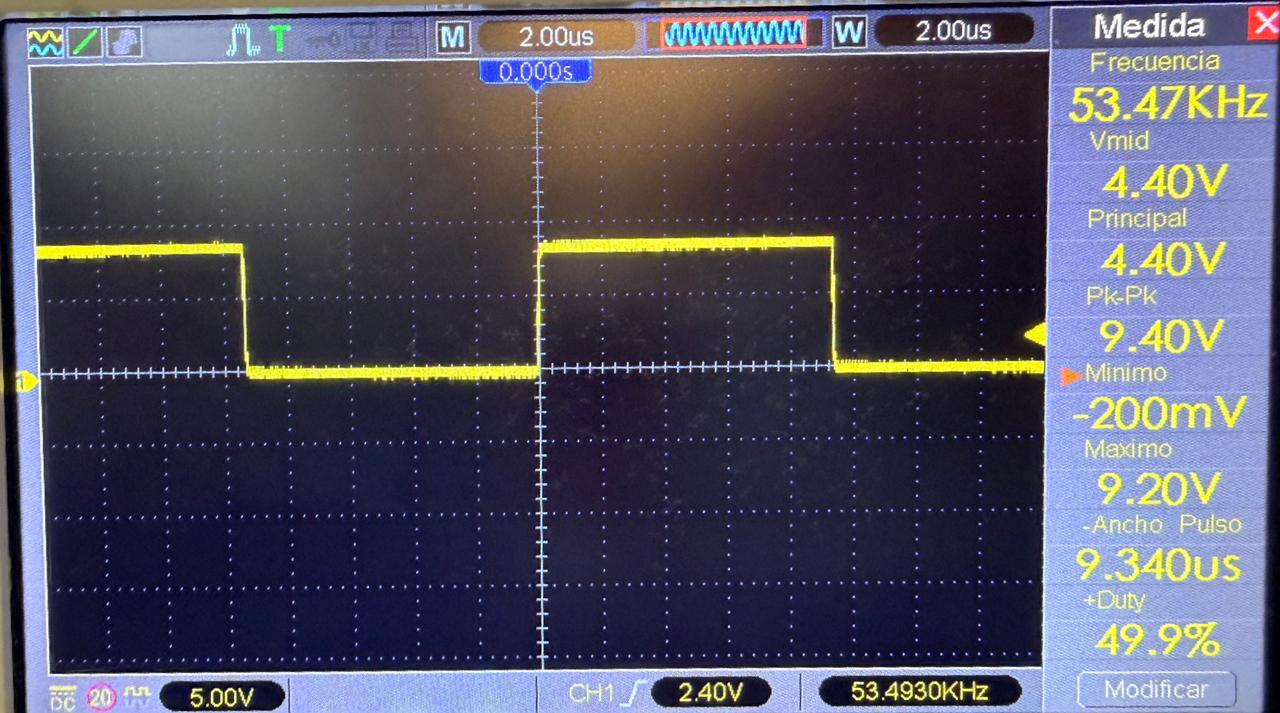
\includegraphics[width=0.8\textwidth]{img/Mediciones imagenes/Entrada GateDriver.png}
    \caption{Señal de entrada del gate Driver.}
    \label{fig:señial entrada gate driver}
\end{figure}

A partir de esta entrada, se obtuvieron, en la Figura~\ref{fig:senial salida gate driver}, las siguientes salidas:

\begin{figure}[H]
    \centering
    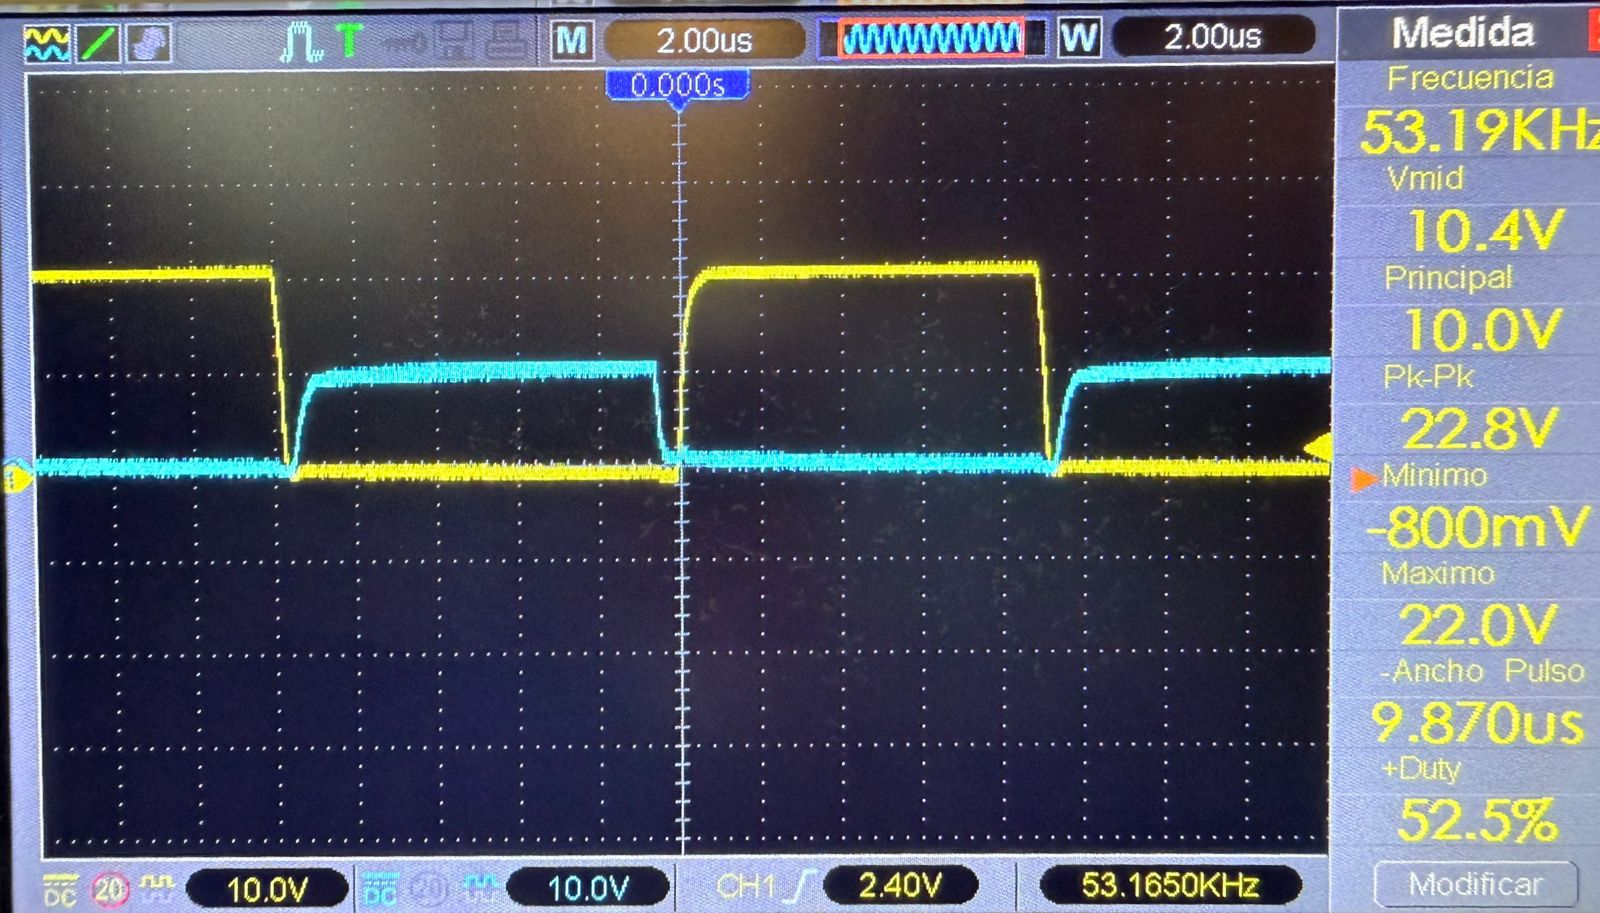
\includegraphics[width=0.9\textwidth]{img/Mediciones imagenes/Salidas GateDriver.jpg}
    \caption{Señales de salida del Gate Driver.}
    \label{fig:senial salida gate driver}
\end{figure}

La diferencia de amplitud entre ambas señales se debe a la forma en que se 
referencian las salidas del Gate Driver. La salida del transistor inferior está 
referida a masa, por lo que conmuta aproximadamente entre $0$ y la tensión de 
alimentación del driver. En cambio, la salida del transistor superior está 
referida al nodo conmutado de la etapa de potencia. Por este motivo, al medirla 
respecto de masa, su tensión incluye tanto la tensión del nodo conmutado como 
la tensión de excitación de compuerta.

Por lo tanto, que una de las señales aparezca con una amplitud mayor no implica 
una amplificación real de la señal de entrada, sino que es consecuencia de medir 
una salida flotante respecto de masa.

Por otro lado, se realizó también la medición del tiempo muerto.

\begin{figure}[H]
    \centering
    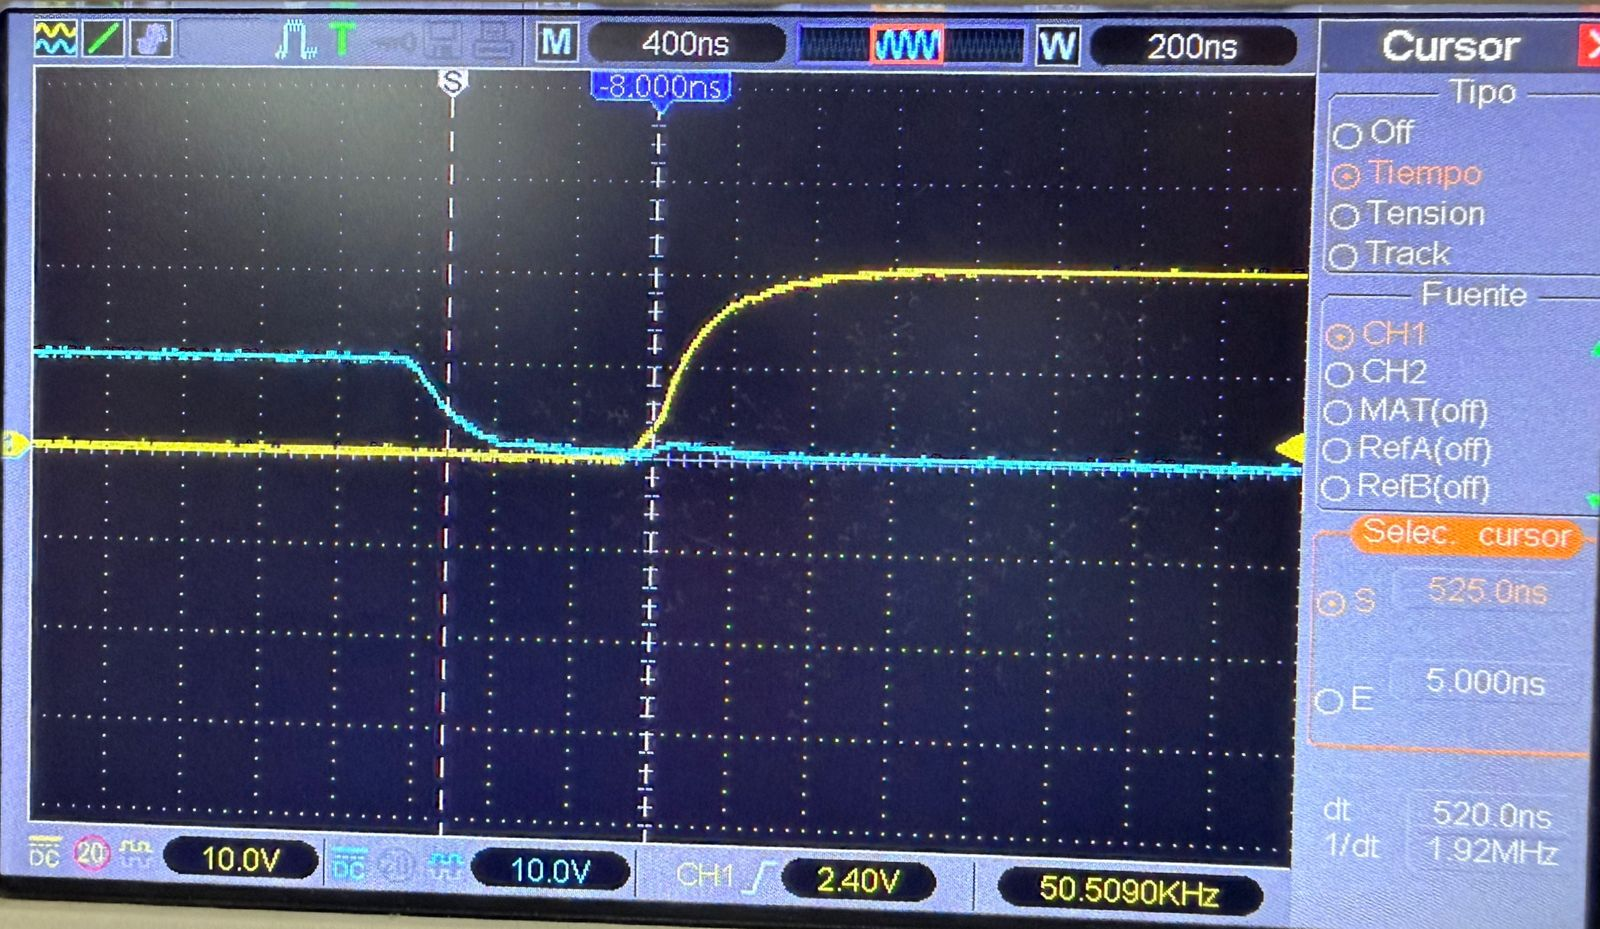
\includegraphics[width=0.9\textwidth]{img/Mediciones imagenes/Tiempo muerto GateDriver.jpg}
    \caption{Tiempo muerto del Gate Driver medido con el osciloscopio.}
    \label{fig:tiempo muerto gate driver}
\end{figure}

En la Figura~\ref{fig:tiempo muerto gate driver} se midió el tiempo muerto del componente en $\SI{520}{\nano\second}$ el cual corresponde al especificado en la hoja de datos del mismo (ver referencias).


\subsection{Conmutación de la \textit{buck}}

Para verificar el funcionamiento de la etapa de potencia se midieron las formas de onda del nodo de conmutación y de la tensión sobre el inductor. Estas mediciones permiten comprobar que las llaves conmutan correctamente y que el inductor alterna entre los intervalos de almacenamiento y entrega de energía propios de un convertidor \textit{buck}.

\begin{figure}[H]
    \centering
    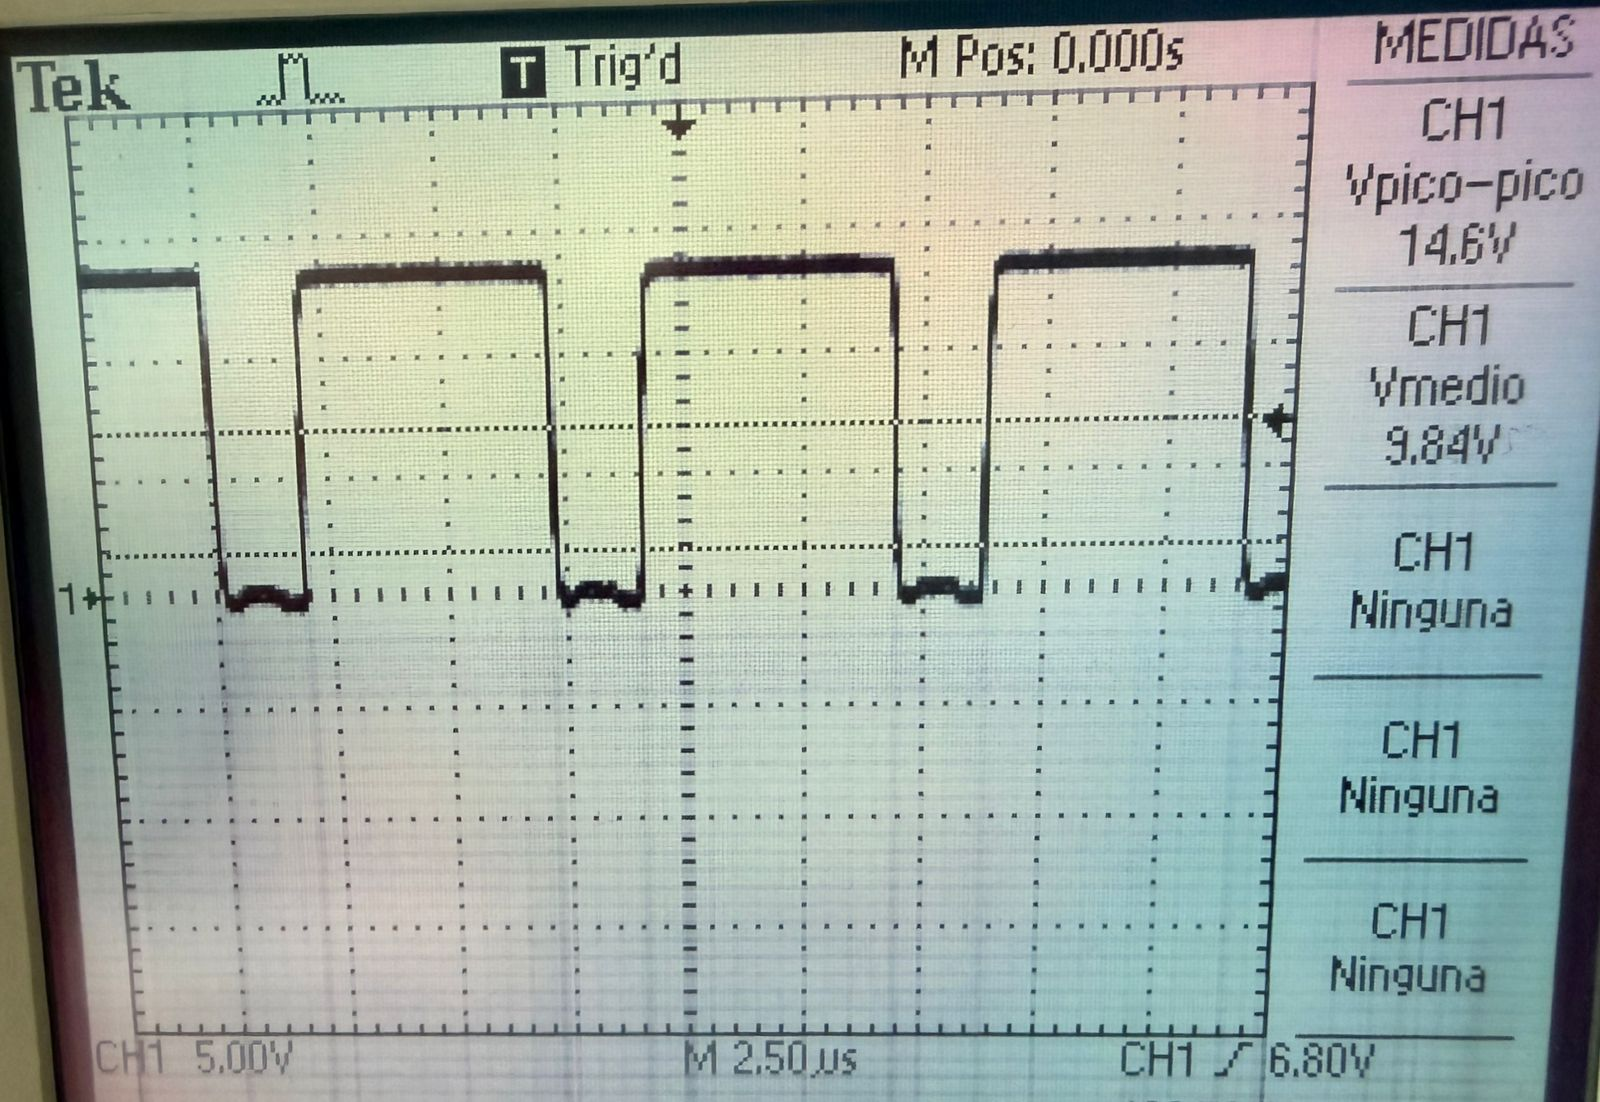
\includegraphics[width=0.8\textwidth]{img/Mediciones imagenes/nodo_conm.jpg}
    \caption{Tensión medida en el nodo de conmutación de la \textit{buck}.}
    \label{fig:nodo_conm}
\end{figure}

En la Figura~\ref{fig:nodo_conm} se observa la tensión del nodo de conmutación. La forma de onda alterna entre un nivel alto, correspondiente al intervalo en que conduce la llave superior, y un nivel bajo, asociado al intervalo de rueda libre. También se aprecian transitorios rápidos en los flancos de conmutación, esperables debido a las capacidades e inductancias parásitas de la etapa de potencia.

\begin{figure}[H]
    \centering
    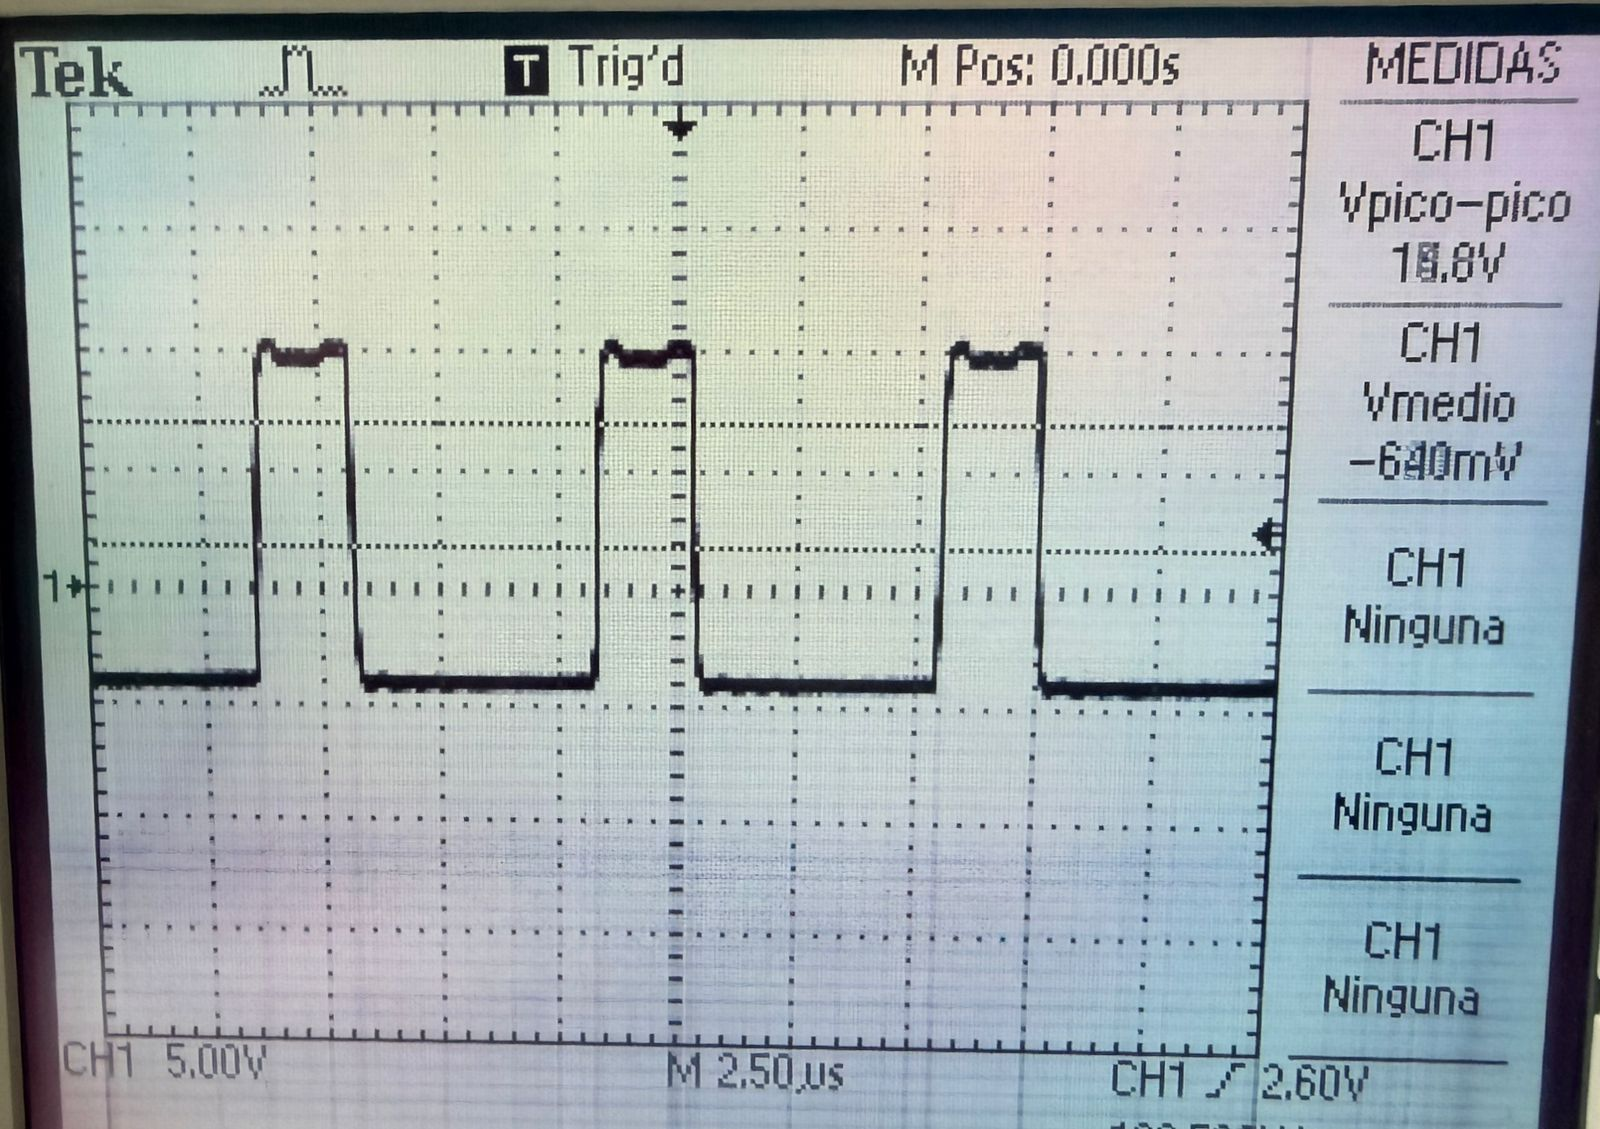
\includegraphics[width=0.8\textwidth]{img/Mediciones imagenes/tension_inductor.jpg}
    \caption{Tensión medida sobre el inductor de la \textit{buck}.}
    \label{fig:tension_inductor}
\end{figure}

En la Figura~\ref{fig:tension_inductor} se muestra la tensión sobre el inductor. Durante el intervalo de conducción de la llave superior, la tensión sobre el inductor es positiva y su corriente aumenta. Durante el intervalo de rueda libre, la tensión cambia de polaridad y la corriente del inductor disminuye. Este comportamiento confirma la transferencia periódica de energía entre la entrada, el inductor y la carga.

\subsection{Eficiencia}
Se midió la eficiencia de la fuente \textit{buck} para diferentes condiciones de carga y tensión de entrada.

\begin{figure}[H]
    \centering
    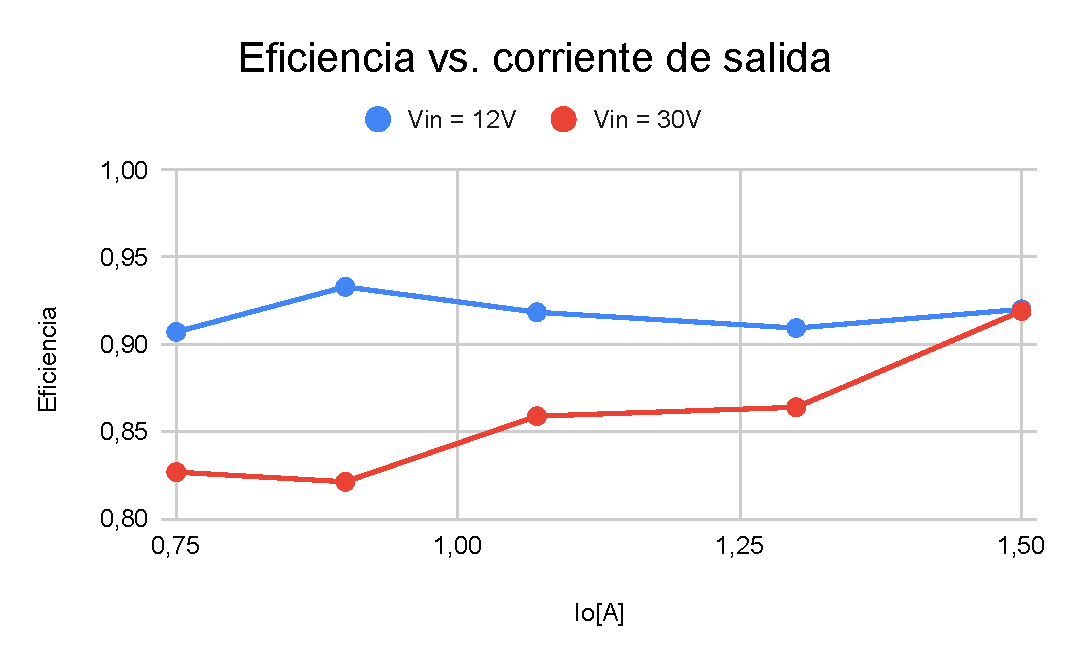
\includegraphics[width=0.8\textwidth]{img/Mediciones imagenes/Eficiencia vs. corriente de salida.pdf}
    \caption{Eficiencia en función de la corriente de salida.}
    \label{fig:ef vs. Io}
\end{figure}

La \autoref{fig:ef vs. Io} muestra la variación de la eficiencia con la corriente de salida para dos tensiones de entrada. Para la curva azul se destaca que en todos los casos la eficiencia fue superior a $90\,$\% y que la misma no varía de forma apreciable con la corriente de salida. Para la curva roja se observa que la eficiencia es menor y que tiende a subir con la corriente de salida. Esto se explica ya que la potencia disipada los reguladores utilizados para alimentar al PWM, a la red de compensación y al \textit{gate driver} aumenta con la tensión de entrada, ya que la caída de tensión en dichos reguladores es mayor. 

\begin{figure}[H]
    \centering
    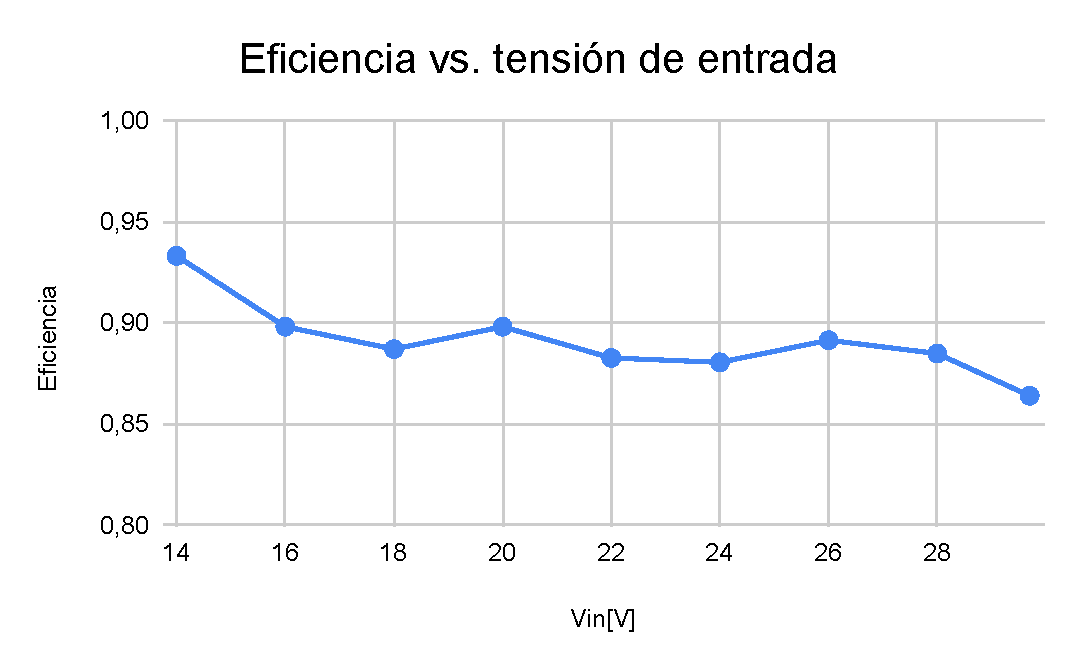
\includegraphics[width=0.8\textwidth]{img/Mediciones imagenes/Eficiencia vs. tensión de entrada.pdf}
    \caption{Eficiencia en función de la tensión de entrada.}
    \label{fig:ef vs. Vin}
\end{figure}

La \autoref{fig:ef vs. Vin} muestra la variación de la eficiencia con la tensión de entrada a una corriente de carga constante $I_o = \SI{0.75}{\ampere}$ . Se destaca que en todos los casos la eficiencia fue superior a $85\,$\% y que la misma decrece ligeramente a mayor tensión de entrada. Esto se debe a que la potencia de salida se mantiene constante (ya que no varía la tensión de salida ni la corriente de salida), mientras que la potencia de entrada aumenta, por lo que el cociente $\eta = \frac{P_O}{P_{IN}}$ disminuye. 

\subsection{Regulación de línea y carga}

\begin{figure}[H]
    \centering
    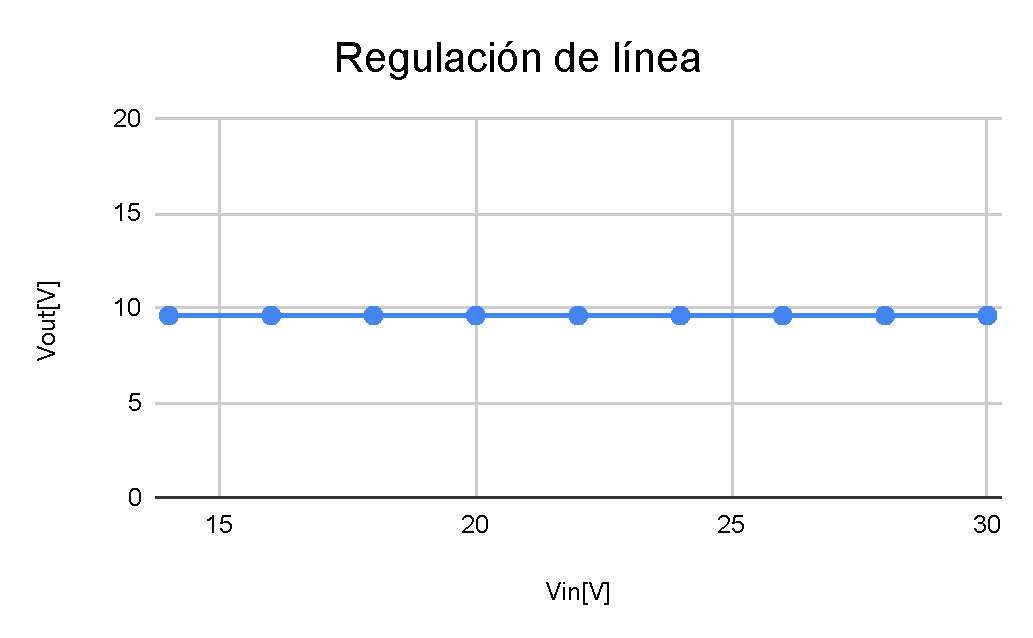
\includegraphics[width=0.8\textwidth]{img/Mediciones imagenes/Regulación de linea.pdf}
    \caption{Regulación de línea.}
    \label{fig:RegLin}
\end{figure}

La \autoref{fig:RegLin} muestra los puntos obtenidos en la medición de la regulación de línea, la cual fue hecha con un osciloscopio ya que la resolución del multímetro resultó insuficiente. Se observó que la tensión de salida apenas varía ante cambios en la tensión de entrada y que esta variación es tan pequeña que no pudo ser apreciada por el multímetro. Se obtuvo entonces $REG_{LIN} = \SI{0.125}{\milli \volt / volt}$.


Por otro lado, para analizar la regulación de carga se midió la tensión de salida $V_o$ 
variando la resistencia de carga $R_L$. Al disminuir esta, la corriente de 
salida aumentó desde $0{.}75\,\text{A}$ hasta $1{.}5\,\text{A}$.

\begin{figure}[H]
    \centering
    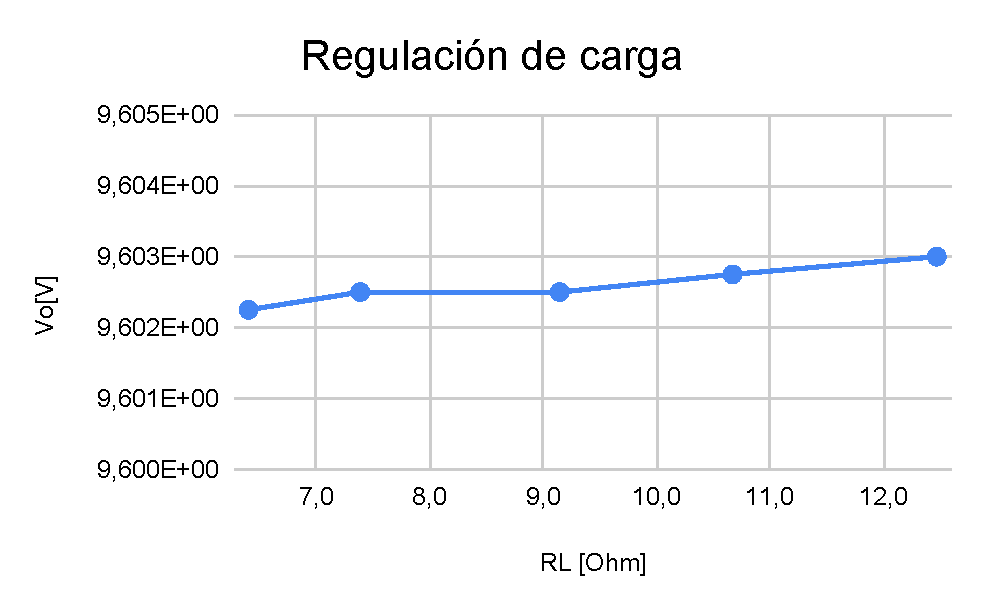
\includegraphics[width=0.8\textwidth]{img/Mediciones imagenes/Regulación de carga.pdf}
    \caption{Regulación de carga}
    \label{fig:RegCar}
\end{figure}

En la fig. \ref{fig:RegCar} se muestra la regulación de carga de la fuente. 
Para esto se midió la tensión de salida \(V_o\) para distintos valores de 
corriente de carga \(I_o\), variando la resistencia \(R_L\).

Se observa que la tensión de salida se mantiene prácticamente constante alrededor 
de \(9{.}6\,\text{V}\), incluso cuando la corriente aumenta desde 
\(0{.}77\,\text{A}\) hasta \(1{.}5\,\text{A}\). Para cuantificar esta variación, 
se calcula la regulación de carga como la pendiente de la recta \(V_o\) en 
función de \(I_o\):

\[
R_{\text{reg}} =
\left|\frac{\Delta V_o}{\Delta I_o}\right|.
\]

Tomando dos puntos de la recta medida,

\[
(I_{o1},V_{o1})=(1{.}3\,\text{A},9{.}6025\,\text{V})
\]

\[
(I_{o2},V_{o2})=(1{.}5\,\text{A},9{.}60225\,\text{V}),
\]

se obtiene

\[
R_{\text{reg}} =
\left|\frac{9{.}60225-9{.}6025}{1{.}5-1{.}3}\right|
=
1{.}25\,\text{m}\Omega.
\]

Este valor es muy bajo, lo que indica que la fuente tiene una buena regulación 
de carga. Es decir, al aumentar la corriente demandada por la carga, la tensión 
de salida prácticamente no cambia.

\subsection{\textit{Ripple} de la tensión de salida}

Como se mencionó en secciones anteriores, el hecho de que el capacitor de salida no se comporte como en la teoría a nuestra frecuencia de operación impidió que el mismo integre eficientemente su corriente, obteniendo un \textit{ripple} lineal en la tensión de salida de la \textit{buck}, tal y como se muestra en la Figura~\ref{fig:ripple_lineal}.

\begin{figure}[H]
    \centering
    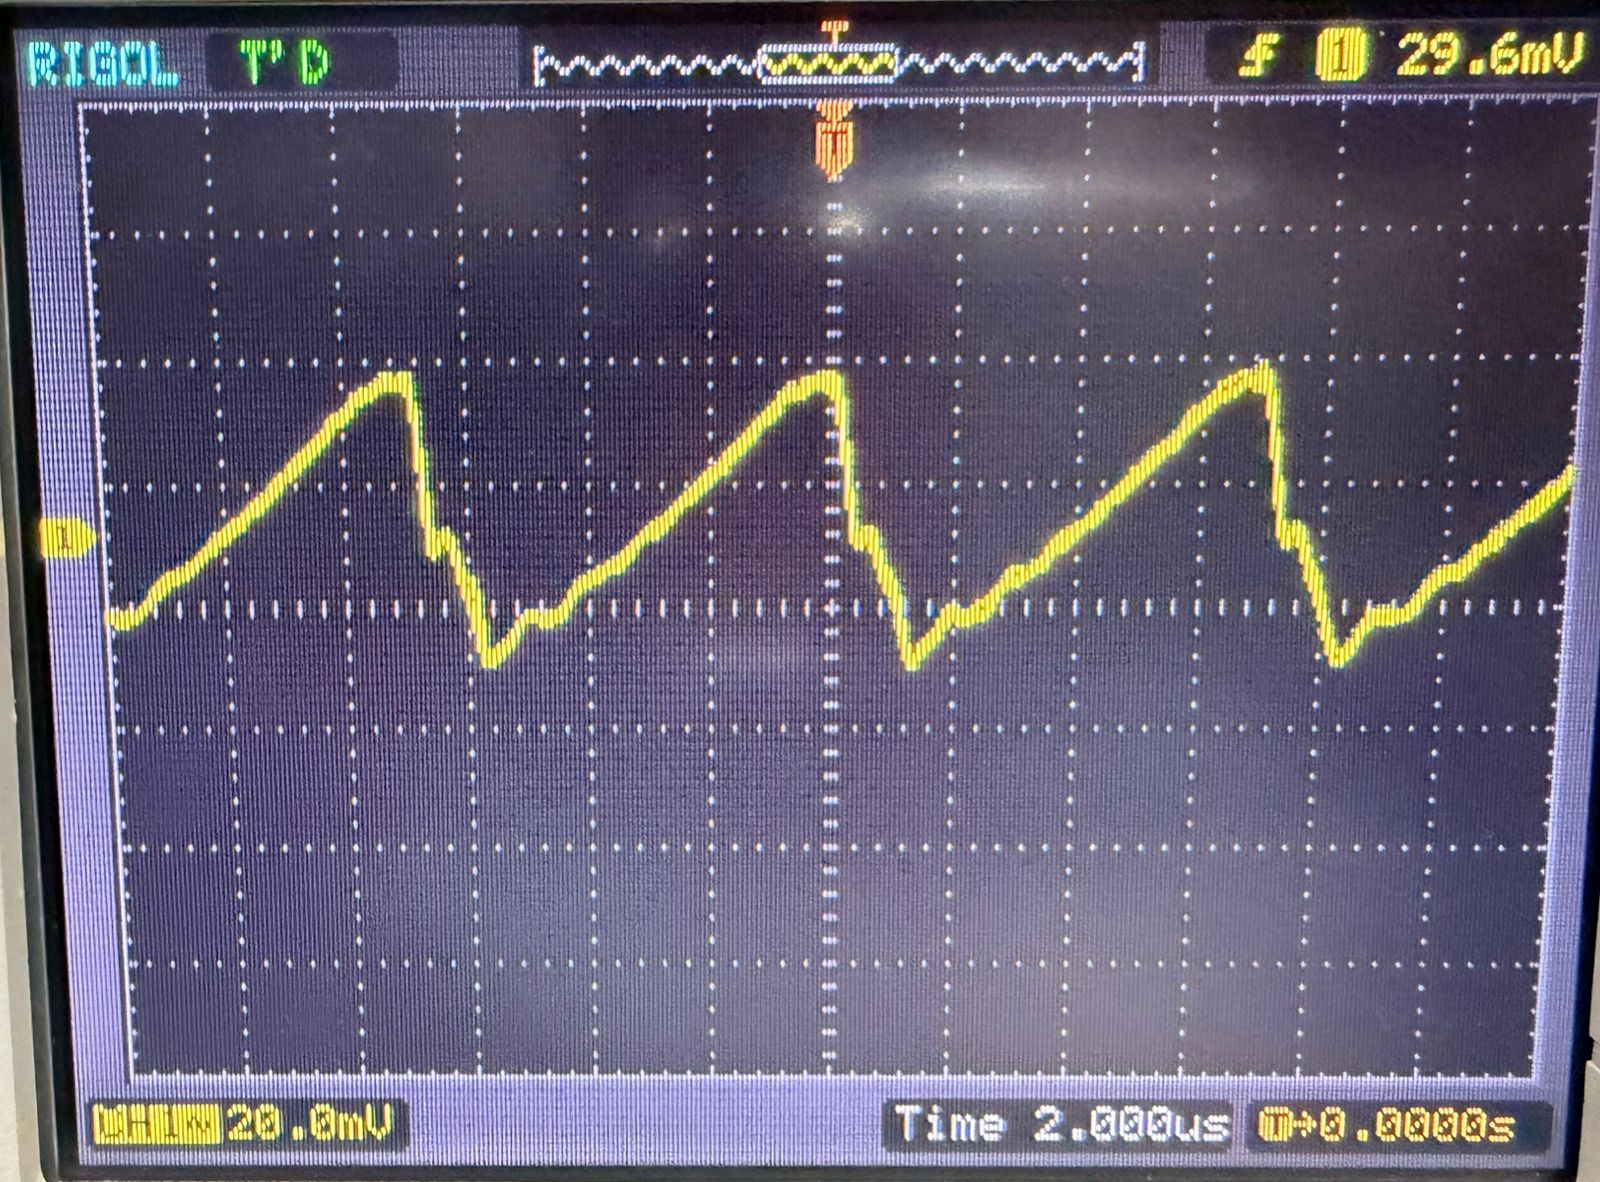
\includegraphics[width=0.8\textwidth]{img/Mediciones imagenes/Salida triangular.jpg}
    \caption{\textit{Ripple} lineal en la tensión de salida de la \textit{buck}.}
    \label{fig:ripple_lineal}
\end{figure}

Para corregir esto se modificó el capacitor de salida de $10\,\upmu$F de una tecnología electrolítica a una cerámica multicapa, la cual no pierde capacitancia a altas frecuencias, permitiendo que el mismo integre correctamente su corriente y obteniendo un \textit{ripple} de tensión cuadrático a la salida de la \textit{buck}, tal y como predice el diseño teórico y como se muestra en la Figura~\ref{fig:ripple_cuad}.

\begin{figure}[H]
    \centering
    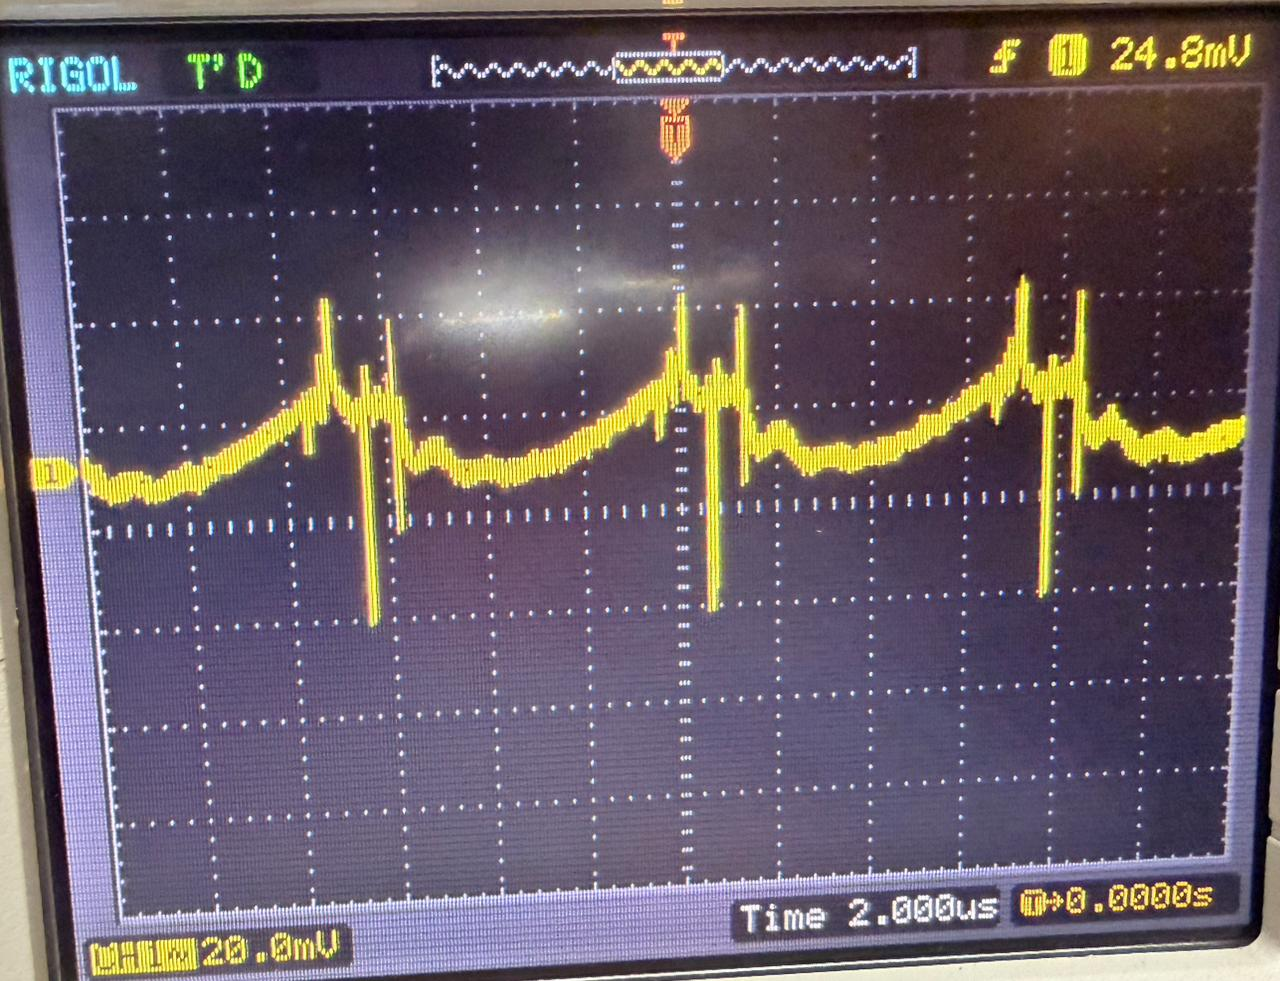
\includegraphics[width=0.8\textwidth]{img/Mediciones imagenes/Salida cuadratica.jpg}
    \caption{\textit{Ripple} cuadrático en la tensión de salida de la \textit{buck}.}
    \label{fig:ripple_cuad}
\end{figure}